\section{Desarrollo del backend}
\subsection{Configuración del entorno}

Para la implementación del backend se configuró un entorno orientado a garantizar estabilidad, reproducibilidad y compatibilidad con los distintos servicios necesarios para el funcionamiento del prototipo. Este entorno se construyó sobre Python 3.11 y empleó un sistema de gestión de dependencias que permitió mantener versiones consistentes de librerías, asegurar un aislamiento apropiado y facilitar el despliegue en múltiples entornos de ejecución.
\\
\\
En esta etapa se configuraron los elementos fundamentales del backend, entre ellos:

\begin{itemize}
    \item \textbf{FastAPI como framework principal:} seleccionado por su rendimiento, asincronía nativa y capacidad para estructurar APIs de manera modular, manteniendo un alto nivel de claridad y escalabilidad en los controladores expuestos al frontend.

    \item \textbf{Gestión de dependencias mediante Poetry:} utilizada para administrar el entorno virtual del proyecto, asegurar versiones específicas de paquetes y garantizar reproducibilidad durante las fases de desarrollo, pruebas y despliegue.

    \item \textbf{Manejo de asincronía en el framework:} aunque FastAPI ofrece soporte nativo para ejecución asincrónica, la implementación actual utiliza principalmente operaciones síncronas tanto en el acceso a la base de datos como en los servicios auxiliares.

    \item \textbf{CORS como mecanismo de interoperabilidad:} configurado para permitir la comunicación segura entre el cliente web y el backend, controlando los orígenes autorizados durante la interacción entre módulos.
\end{itemize}

\subsection{Arquitectura y organización}
 Para la implementación del backend se empleó una arquitectura monolítica modular organizada por capas, un enfoque adecuado para prototipos que requieren simplicidad operativa y una separación clara de responsabilidades. Bajo este esquema, el sistema se estructura en capas diferenciadas (exposición de API, lógica de negocio, acceso a datos e integración con servicios externos) que trabajan de manera coordinada dentro de una misma aplicación.

\subsubsection{Capa de exposición o API}
Corresponde al punto de entrada de todas las solicitudes provenientes del frontend. En esta capa se gestionan aspectos como:

\begin{itemize}
    \item Recepción de peticiones HTTP.
    \item Validación de los datos de entrada.
    \item verificación de autenticación mediante tokens JWT.
    \item Estandarización de los datos de respuesta.
\end{itemize}

La API actúa únicamente como un intermediario: procesa las solicitudes de forma superficial y delega la lógica principal a la capa de servicios, donde se ejecutan las reglas y operaciones del sistema. Este enfoque permite mantener controladores livianos, fáciles de mantener y coherentes con buenas prácticas de desarrollo.

\subsubsection{Capa de servicios o lógica de negocio}
En esta capa se concentra el núcleo del comportamiento del sistema. Aquí se implementan las reglas específicas de cada módulo, así como operaciones complejas que requieren coordinar múltiples entidades y fuentes de datos. Entre sus responsabilidades se incluyen:

\begin{itemize}
    \item Validación de reglas de negocio.
    \item Gestión de transacciones.
    \item Coordinación entre bases de datos relacionales y documentos NoSQL.
    \item Actualizaciones en cascada (por ejemplo, el estado de un objetivo según el progreso de sus tareas).
    \item Orquestación de procesos que combinan datos, IA y almacenamiento externo.
\end{itemize}

La lógica del módulo \textit{Aprender a Aprender} se construyó sobre servicios responsables de manejar metas, objetivos y tareas, mientras que el módulo \textit{Escucha Activa} incorpora servicios especializados para administrar sesiones de juego, rondas, desafíos, evaluación y generación de audio.

\subsubsection{Capa de acceso a datos}
Esta capa define el mecanismo mediante el cual los servicios interactúan con las bases de datos. El prototipo combina:

\begin{itemize}
    \item \textbf{PostgreSQL}, utilizado para almacenar información estructurada como usuarios, metas, objetivos, tareas, sesiones de juego, rondas y desafíos.
    \item \textbf{MongoDB}, empleado para representar estructuras jerárquicas completas (por ejemplo, un learning goal con todos sus objetivos y tareas) y para gestionar los roadmaps generados mediante IA.
\end{itemize}

Mientras PostgreSQL garantiza integridad referencial y transacciones ACID, MongoDB ofrece flexibilidad y acceso eficiente a documentos completos. La sincronización entre ambas fuentes de datos permite aprovechar las fortalezas de cada una sin duplicar lógica innecesariamente.

\subsubsection{Capa de integración con servicios externos}
Algunas funcionalidades centrales del prototipo dependen de servicios especializados, entre ellos:

\begin{itemize}
    \item \textbf{Modelos de lenguaje (OpenAI + LangChain):} utilizados para generar desafíos auditivos, construir prompts dinámicos, evaluar las respuestas proporcionadas por los participantes y procesar salidas estructuradas mediante esquemas validados.

    \item \textbf{Síntesis de voz (ElevenLabs):} responsable de convertir el contenido textual de los desafíos en audio, empleando voces configurables y modelos multilingües.

    \item \textbf{Almacenamiento en la nube (Supabase Storage):} utilizado para guardar de manera persistente los archivos de audio generados y exponerlos mediante URLs públicas accesibles desde el cliente.
\end{itemize}

Esta capa permite encapsular las interacciones con servicios externos y abstraer su complejidad del resto del sistema.

\subsection{Visión general de componentes}

El backend se encuentra organizado en un conjunto de componentes que estructuran las
funcionalidades del sistema y facilitan la separación de responsabilidades. Estos componentes
están organizados en los directorios principales del proyecto y actúan como bloques funcionales que
permiten gestionar modelos de datos, lógica de negocio, validaciones, acceso a bases de datos y
servicios externos.
\\
\\
Tanto la estructura de carpetas como la descripción de cada componente se presentan en la
Figura~\ref{fig:estructura_backend_textual} y en la Tabla~\ref{tab:componentes_backend},
respectivamente.

\begin{figure}[H]
\centering
\begin{verbatim}
backend/
|-- alembic/                 (Migraciones para la base de datos PostgreSQL)
|-- data/                    (Recursos estáticos y archivos auxiliares)
|-- enums/                   (Enumeraciones del sistema: estados, tipos y constantes)
|-- llm/                     (Integración con modelos de lenguaje y generación de contenidos)
|-- model/                   (Modelos SQLModel para PostgreSQL)
|-- mongo_service/           (Servicios para operaciones con MongoDB)
|-- nosql_models/            (Modelos de documentos NoSQL)
|-- nosql_schema/            (Esquemas de validación para documentos en MongoDB)
|-- router/                  (Endpoints de la API organizados por dominio funcional)
|-- schema/                  (Esquemas Pydantic para validación y respuesta)
|-- service/                 (Lógica de negocio y orquestación de procesos)
+-- utils/                   (Funciones auxiliares y utilidades compartidas)
\end{verbatim}
\caption{Estructura jerárquica de directorios del backend. Elaboración propia.}
\label{fig:estructura_backend_textual}
\end{figure}


\begin{table}[H]
\centering
\footnotesize
\setlength{\tabcolsep}{8pt}
\renewcommand{\arraystretch}{1.25}
\begin{tabular}{|p{3cm}|p{11cm}|}
\hline
\textbf{Componente} & \textbf{Descripción} \\
\hline

\textbf{alembic} &
Gestiona las migraciones del esquema de PostgreSQL. Incluye configuraciones, plantillas y
versiones que permiten crear o modificar tablas, columnas y restricciones de forma controlada. \\
\hline

\textbf{data} &
Contiene scripts de inicialización y carga de datos de prueba (\textit{seed}), utilizados durante el
desarrollo para poblar PostgreSQL y MongoDB con usuarios, metas, objetivos y otros elementos
del prototipo. \\
\hline

\textbf{enums} &
Contiene las enumeraciones que representan valores fijos del backend, incluyendo modos de juego, estados de sesión, roles de usuario, tipos de recurso y otros valores tipados utilizados a lo largo del sistema. \\
\hline

\textbf{llm} &
Implementa la integración con modelos de lenguaje mediante LangChain y OpenAI. Incluye
clientes de LLM, generadores de desafíos auditivos, evaluadores de respuestas y cargadores de
prompts utilizados en el módulo de Escucha Activa. \\
\hline

\textbf{model} &
Define los modelos de datos persistentes basados en SQLModel, que representan tablas y
relaciones en PostgreSQL. Contiene entidades como usuarios, metas, objetivos, tareas, sesiones
de juego, rondas y desafíos. \\
\hline

\textbf{mongo\_service} &
Incluye servicios especializados para operar sobre MongoDB, gestionando documentos
jerárquicos asociados a metas, objetivos, tareas y roadmaps. Facilita la sincronización dual entre
PostgreSQL y la base documental. \\
\hline

\textbf{nosql\_models} &
Modelos Pydantic que representan la estructura de documentos almacenados en MongoDB,
particularmente para los roadmaps y sus componentes anidados. \\
\hline

\textbf{nosql\_schema} &
Esquemas para validar, serializar y convertir documentos NoSQL en modelos tipados. Proveen
el formato de entrada y salida en operaciones relacionadas con roadmaps. \\
\hline

\textbf{router} &
Expone los endpoints REST del backend. Cada archivo corresponde a un dominio funcional como
autenticación, metas, objetivos, tareas, roadmaps, desafíos o sesiones de juego. Los routers se encargan de recibir las solicitudes, aplicar las validaciones de entrada necesarias,
gestionar la autenticación y delegar la ejecución al nivel de servicios.
\\
\hline

\textbf{schema} &
Define los esquemas Pydantic utilizados para validar datos de entrada y estructurar las
respuestas de la API. Incluye schemas de creación, actualización, paginación y respuestas
especializadas para cada módulo. \\
\hline

\textbf{service} &
Implementa la lógica de negocio del sistema. Coordina operaciones entre modelos, gestiona reglas
de negocio, orquesta transacciones en PostgreSQL y sincroniza datos con MongoDB, además de
interactuar con servicios externos como OpenAI, ElevenLabs y Supabase Storage. \\
\hline

\textbf{utils} &
Contiene utilidades compartidas: configuración del sistema, clientes de PostgreSQL y MongoDB,
integraciones con almacenamiento y síntesis de voz, serializadores, validadores y funciones de
apoyo utilizadas en múltiples módulos. \\
\hline

\end{tabular}
\caption{Visión general de los componentes del backend}
\label{tab:componentes_backend}
\end{table}

\subsection{Diagramas de arquitectura}

Con el fin de complementar la descripción de la arquitectura presentada previamente, se incluyen diagramas detallados para cada uno de los componentes principales del sistema. Estos diagramas ilustran el flujo de interacción entre el cliente web, el servidor backend y las bases de datos empleadas, destacando las operaciones de lectura (\textbf{R}) y escritura (\textbf{W}) involucradas en cada funcionalidad.
\\

Cada descripción hace referencia a su respectivo diagrama arquitectónico, disponible en el \textbf{Anexo F}. Para mantener claridad y evitar redundancia, se mencionan únicamente las operaciones generales asociadas a cada componente, mientras que la definición completa de los endpoints puede consultarse en el \hyperref[anexo:endpoints]{\textbf{Anexo H}}.

\subsubsection{Gestión de metas de aprendizaje}

El componente encargado de la gestión de metas maneja operaciones de creación, consulta, actualización y eliminación de metas definidas por el usuario. Estas operaciones se realizan mediante solicitudes recibidas en la API y delegadas a los servicios correspondientes, los cuales coordinan la persistencia en PostgreSQL (\textbf{R/W}) y la sincronización con MongoDB para mantener la estructura jerárquica completa.
\\

El flujo detallado de esta interacción se presenta en el \hyperref[fig:anexoF-learning-goals]{\textbf{Anexo F.1}}.

\subsubsection{Gestión de objetivos}

El componente de objetivos permite administrar los elementos intermedios que estructuran cada meta. Incluye operaciones para crear objetivos, actualizar su estado, reorganizarlos y consultarlos de manera individual o agrupada. Estas operaciones se reflejan en PostgreSQL (\textbf{R/W}) y se sincronizan en MongoDB para garantizar una representación completa y eficiente en las interfaces.
\\

El diagrama asociado a este componente se encuentra en el \hyperref[fig:anexoF-objectives]{\textbf{Anexo F.2}}.

\subsubsection{Gestión de tareas}

Este componente gestiona las tareas asociadas a cada objetivo e incluye operaciones como creación, actualización de estado, registro de tiempos, modificación de prioridades y eliminación. Además, coordina la actualización del tablero Kanban y sincroniza los cambios en MongoDB para sostener la estructura jerárquica utilizada por la interfaz.
\\

El flujo correspondiente se presenta en el \hyperref[fig:anexoF-tasks]{\textbf{Anexo F.3}}.

\subsubsection{Notas y recursos asociados a tareas}

Las notas y los recursos complementan el seguimiento del aprendizaje y se gestionan como subcomponentes de las tareas. Las operaciones de creación, consulta, actualización y eliminación se registran en PostgreSQL (\textbf{W}) y, cuando aplica, se reflejan en MongoDB para mantener la estructura documental sincronizada.
\\

Los diagramas respectivos se encuentran en el \hyperref[fig:anexoF-task-notes]{\textbf{Anexo F.4}} y el \hyperref[fig:anexoF-task-resources]{\textbf{Anexo F.5}}.

\subsubsection{Autoevaluaciones}

El componente de autoevaluaciones permite registrar reflexiones sobre el proceso de estudio, capturando datos sobre el contexto, las dificultades y los aprendizajes del usuario. Estas operaciones se almacenan íntegramente en PostgreSQL (\textbf{R/W}), dado que no requieren representación jerárquica en MongoDB.
\\

El diagrama que describe este flujo se encuentra en el \hyperref[fig:anexoF-self-evaluations]{\textbf{Anexo F.6}}.

\subsubsection{Roadmaps}

Los roadmaps representan planes de aprendizaje generados o editados por el usuario. El componente permite crear, modificar, visualizar y convertir roadmaps en metas accionables. Cada operación combina escritura en PostgreSQL (\textbf{W}) para la información general y en MongoDB (\textbf{R/W}) para preservar la estructura visual y el layout del diagrama.
\\

El diagrama asociado se presenta en el \hyperref[fig:anexoF-roadmaps]{\textbf{Anexo F.7}}.

\subsubsection{Sesiones de Escucha Activa}

Este componente administra el ciclo completo de una sesión de juego: creación de la sesión, configuración, avance entre rondas, evaluación de respuestas y consolidación de resultados. Las operaciones se almacenan principalmente en PostgreSQL (\textbf{R/W}), dada su naturaleza transaccional.
\\

El diagrama correspondiente se encuentra en el \hyperref[fig:anexoF-listening-sessions]{\textbf{Anexo F.8}}.

\subsubsection{Desafíos auditivos y generación de audio}

Este componente integra los servicios de modelos de lenguaje para generar desafíos auditivos y los servicios de síntesis de voz para producir los audios utilizados durante las sesiones de juego. Incluye operaciones de solicitud al LLM, almacenamiento del audio en la nube y registro del desafío en PostgreSQL (\textbf{W}). La metadata de cada modo de juego se gestiona mediante estructuras flexibles en campos \texttt{JSONB}.
\\

(No cuenta con un diagrama independiente, pues su flujo se encuentra incorporado dentro del diagrama general de sesiones en el \hyperref[fig:anexoF-listening-sessions]{\textbf{Anexo F.8}}.)

\subsection{Diseño de la base de datos}

El prototipo emplea un diseño de base de datos híbrido que combina un modelo relacional,
soportado en PostgreSQL, y un modelo documental basado en MongoDB. Esta arquitectura permite
gestionar información estructurada y, al mismo tiempo, manejar representaciones jerárquicas y
layouts utilizados en los módulos del sistema.

\subsubsection{Modelo relacional (PostgreSQL)}

La base de datos relacional tiene como objetivo gestionar la información estructurada de los
usuarios, sus metas de aprendizaje y las actividades asociadas a los módulos de Aprender a
Aprender y Escucha Activa. 
\\
\\
A continuación, se presenta una descripción breve de las tablas principales:

\begin{itemize}
  \item \textbf{users}: almacena la información básica de los usuarios del sistema, incluyendo
  credenciales, rol, estado de la cuenta y marcas de auditoría (fechas de creación, actualización y
  último acceso).

  \item \textbf{learning\_goals}: registra las metas de aprendizaje definidas por cada usuario, con
  campos para el título, descripción, impacto esperado y el orden personalizado de los objetivos que
  componen cada meta.

  \item \textbf{objectives}: representa los objetivos específicos asociados a una meta de
  aprendizaje. Incluye información sobre estado, prioridad, fechas de inicio y finalización, así
  como una estructura en formato \texttt{JSONB} que organiza las tareas según su estado para
  soportar la vista tipo tablero Kanban.

  \item \textbf{tasks}: contiene las tareas concretas vinculadas a cada objetivo. Registra el tipo de
  tarea, su estado, prioridad, tiempos estimados y reales de dedicación, fechas de seguimiento y un
  indicador para marcar tareas opcionales.

  \item \textbf{task\_notes}: almacena notas y comentarios asociados a una tarea específica, lo que
  permite capturar observaciones, ideas o recordatorios relevantes para el proceso de estudio.

  \item \textbf{task\_resources}: registra los recursos externos relacionados con una tarea, tales
  como artículos, videos o documentos, especificando el tipo de recurso, su título y el enlace de
  acceso.

  \item \textbf{self\_evaluations}: guarda las autoevaluaciones realizadas por el usuario al
  completar una tarea, incluyendo información sobre el contexto de estudio, la percepción de
  dificultad, el nivel de concentración, el estado de ánimo y las reflexiones sobre lo que funcionó
  bien, los desafíos encontrados y el plan de mejora.

  \item \textbf{pomodoro\_preferences}: almacena las preferencias personalizadas de la técnica
  Pomodoro para cada usuario (duración de los intervalos de trabajo y descanso, ciclos, volumen y
  configuración de sonido), utilizadas para estimar y registrar el tiempo dedicado a las tareas.

  \item \textbf{listening\_game\_session}: representa una sesión de juego del módulo de
  \textit{Escucha Activa}. Registra el usuario asociado, el nombre de la sesión, su estado, la ronda
  actual, la puntuación acumulada y las marcas de tiempo de creación, inicio y finalización.

  \item \textbf{listening\_game\_session\_config}: almacena la configuración detallada de cada
  sesión de juego, incluyendo número de rondas, dificultad, modos de juego permitidos, límites de
  tiempo por modo y parámetros de audio, utilizando campos \texttt{JSONB} para mantener una
  configuración flexible.

  \item \textbf{listening\_game\_round}: modela las rondas individuales de una sesión. Cada
  registro indica el número de ronda, el estado, el modo de juego, el tipo de prompt, la
  puntuación obtenida y el desafío asociado, así como las marcas de tiempo que describen su ciclo
  de preparación, inicio y finalización.

  \item \textbf{listening\_challenge}: almacena los desafíos generados mediante modelos de
  lenguaje. Incluye el texto base que se sintetiza a audio, la dificultad, el modo de juego, la
  URL del audio generado y una estructura \texttt{JSONB} que guarda la metadata específica de
  cada modo (por ejemplo, opciones de respuesta, textos de referencia o rúbricas).

  \item \textbf{listening\_round\_submission}: registra las respuestas del usuario en cada ronda,
  incluyendo la carga útil de la respuesta en formato \texttt{JSONB}, la puntuación obtenida, la
  indicación de si fue correcta, el feedback generado y los tiempos de envío. Se aplican
  restricciones de unicidad para garantizar una única respuesta por ronda y soportar mecanismos
  de idempotencia.
\end{itemize}

\subsection{Modelo entidad relación}

En la Figura~\ref{fig:erd} se presenta el modelo entidad–relación que describe la estructura conceptual del sistema, incluyendo las entidades principales y las relaciones entre ellas.

\begin{figure}[H]
    \centering
    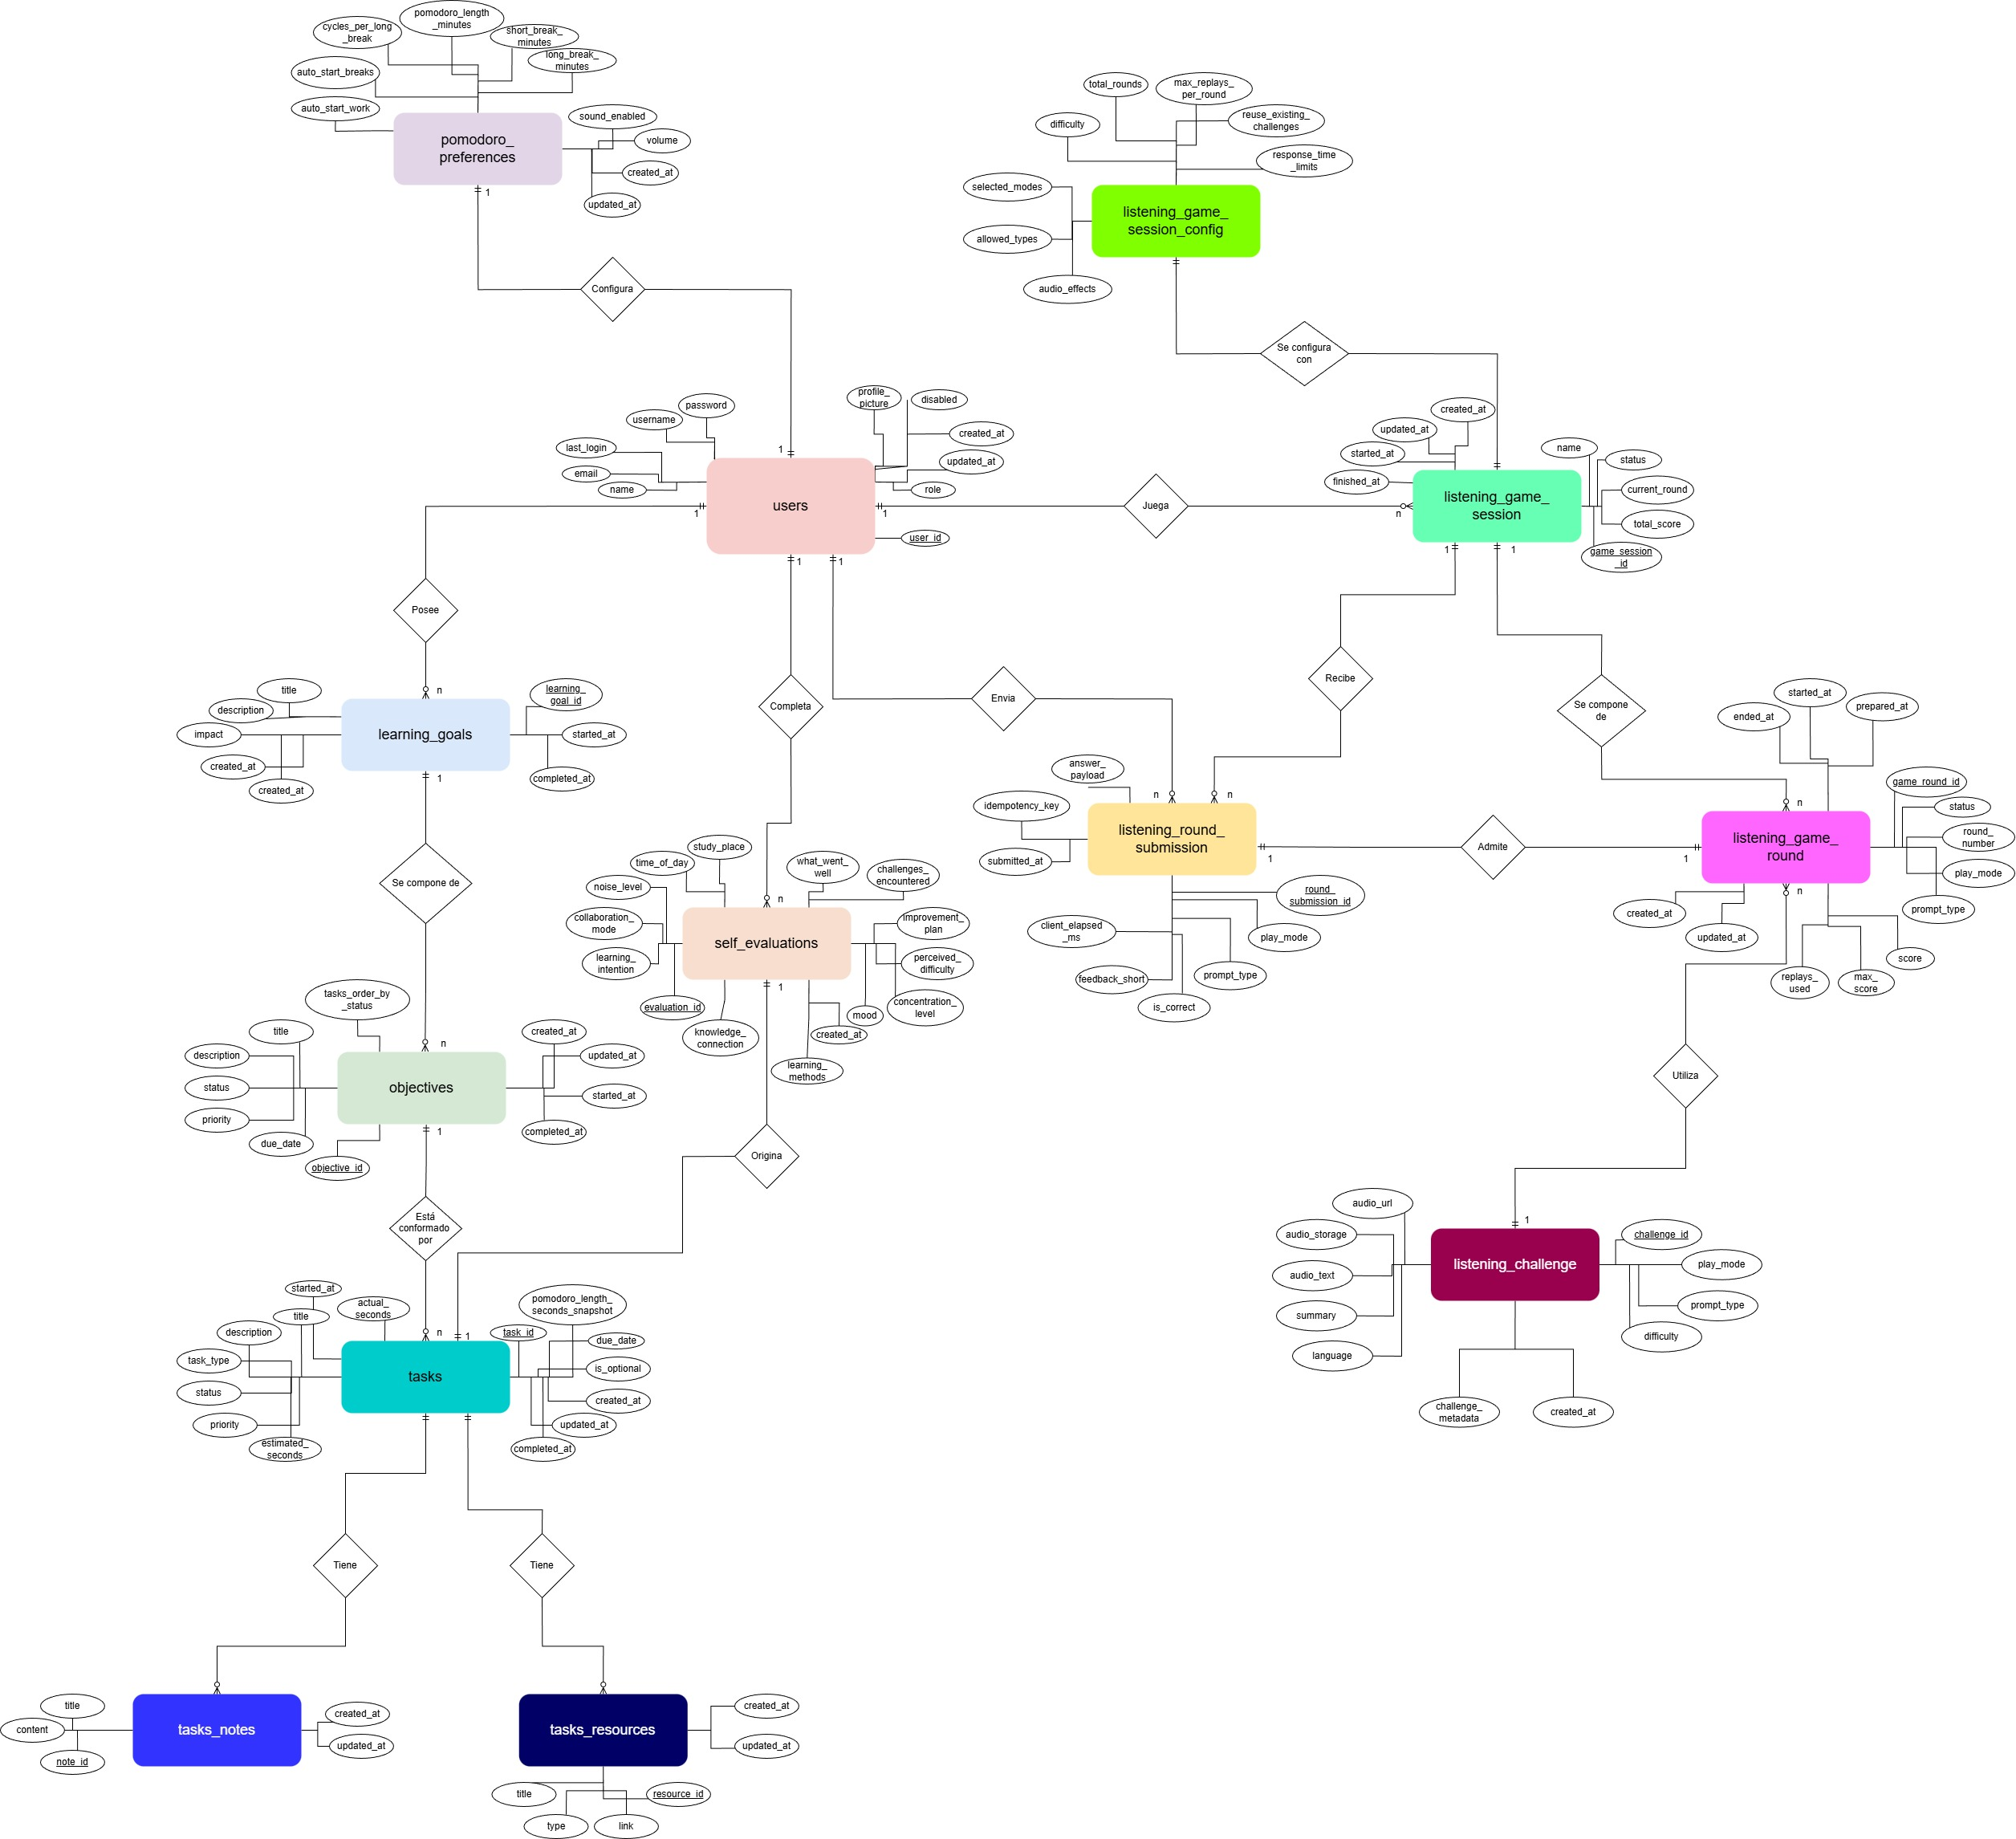
\includegraphics[width=\textwidth]{Figuras/mer_soft_skills_back.jpg} 
    \caption{Modelo entidad–relación. Elaboración propia.}
    \label{fig:erd}
\end{figure}



\subsubsection{Modelo documental (MongoDB)}

El modelo documental complementa al esquema relacional para aquellas funcionalidades que
requieren manejar estructuras jerárquicas completas o layouts visuales. En particular, se emplean
dos colecciones principales: \texttt{learning\_goals} y \texttt{roadmaps}, definidas en bases de datos
separadas para organizar la información persistida en el módulo de Aprender a Aprender y
en el editor de roadmaps.

\begin{itemize}
  \item \textbf{Colección \texttt{learning\_goals}}: almacena documentos que representan una meta
  de aprendizaje con toda su jerarquía de objetivos y tareas anidados. Cada documento replica la
  estructura lógica definida en PostgreSQL, incluyendo el orden de los objetivos y la organización de
  tareas por estado, lo que permite recuperar en una sola consulta la estructura completa que se
  muestra en la interfaz.

  \item \textbf{Colección \texttt{roadmaps}}: guarda los planes de aprendizaje generados y
  compartidos por los usuarios. Además de los objetivos y tareas, incorpora un campo de
  \textit{layout} que registra la posición de los nodos y las aristas del diagrama, permitiendo
  reconstruir la representación visual del roadmap en el editor, así como configurar su visibilidad
  (pública o privada) y la información del autor.
\end{itemize}

\subsubsection{Sincronización y decisiones de diseño}
MongoDB resulta adecuado para almacenar layouts visuales y estructuras jerárquicas que evolucionan
con frecuencia, mientras que PostgreSQL concentra los datos transaccionales del sistema (como
sesiones de juego, rondas, desafíos y envíos de respuestas) donde se requieren transacciones ACID,
restricciones de unicidad e integridad referencial.
\\
\\
Las operaciones de creación, actualización y eliminación sobre metas, objetivos y tareas se ejecutan
inicialmente en PostgreSQL y, de forma coordinada, se reflejan en MongoDB mediante servicios
especializados que serializan los modelos relacionales en documentos. Este esquema de
sincronización dual permite aprovechar las garantías del modelo relacional sin sacrificar la
eficiencia necesaria para recuperar estructuras completas en las visualizaciones del sistema.
\\
\\
La decisión de mantener una representación documental de \texttt{learning\_goals} en MongoDB,
además de su almacenamiento en PostgreSQL, responde a necesidades específicas del módulo
Aprender a Aprender. Las visualizaciones requieren obtener en una única operación la jerarquía
completa de una meta (objetivos, tareas, recursos y su organización tipo Kanban), lo que en un
modelo relacional implicaría múltiples uniones o consultas encadenadas. En MongoDB esta jerarquía
se conserva como un documento anidado, lo que permite su recuperación con baja latencia. 
\\
\\
Asimismo, mantener una representación documental de los planes accionables (\texttt{learning\_goals}) en MongoDB simplifica de manera significativa la conversión entre un roadmap y su versión operativa. Ambas
estructuras (el roadmap y el plan accionable) comparten un formato jerárquico anidado basado
en objetivos y tareas, lo que permite transformarlas entre sí sin necesidad de reconstruir relaciones
mediante consultas complejas.
\\
\\
En la conversión de un plan accionable hacia un roadmap, el sistema recupera desde MongoDB el
documento completo asociado, evitando múltiples consultas o uniones en PostgreSQL para
reconstruir la jerarquía. Dado que el roadmap también se almacena como un documento anidado,
la transformación consiste principalmente en reorganizar la misma estructura de datos para
adaptarla al editor visual.
\\
\\
En sentido inverso, cuando un usuario adopta un roadmap como plan de aprendizaje, el sistema
itera sobre sus objetivos y tareas y crea los registros correspondientes en PostgreSQL. Aunque este
proceso genera nuevas entidades relacionales, la estructura documental del roadmap facilita el
mapeo, pues su jerarquía coincide con la utilizada por los planes accionables almacenados en
MongoDB. Posteriormente, el servicio de sincronización actualiza la versión documental,
garantizando coherencia entre ambos modelos persistidos.
\\
\\
Finalmente, el uso de campos JSONB, arreglos ordenados e índices compuestos en PostgreSQL
(especialmente en entidades como \texttt{objectives}, \texttt{tasks} y \texttt{listening\_game\_round})
complementa el modelo documental al permitir almacenar configuraciones flexibles y optimizar
consultas comunes sobre combinaciones de columnas (por ejemplo, \texttt{objective\_id} y
\texttt{status}, o \texttt{session\_id} y \texttt{round\_number}). En conjunto, la complementariedad entre
PostgreSQL y MongoDB permite combinar integridad, flexibilidad y rendimiento en las operaciones
propias de los módulos de Aprender a Aprender y Escucha Activa.


\subsubsection{Modelos de datos y validaciones}

El backend representa la información persistida mediante tres tipos de estructuras:
\begin{enumerate}[label=(\roman*), leftmargin=*]
    \item Modelos ORM basados en \texttt{SQLModel} para las entidades gestionadas en PostgreSQL.
    \item Esquemas de validación definidos con \texttt{Pydantic} para las operaciones de la API REST. 
    \item Modelos \texttt{Pydantic} utilizados para representar documentos almacenados en MongoDB.
\end{enumerate}
Los modelos construidos con \texttt{SQLModel} (que combinan las capacidades de 
\texttt{SQLAlchemy} y \texttt{Pydantic}) definen la estructura interna de las entidades 
persistidas en PostgreSQL. Por su parte, los esquemas Pydantic complementan esta 
definición mediante validaciones adicionales aplicadas durante el intercambio de datos 
con la API. Entre los elementos más relevantes se encuentran:

\begin{itemize}
    \item \textbf{Modelos SQLModel}: definen campos tipados, relaciones mediante 
    \texttt{Relationship}, configuraciones de persistencia y validaciones básicas que 
    reflejan de manera directa el esquema relacional.
    
    \item \textbf{Esquemas Pydantic}: incorporan restricciones de formato, valores por 
    defecto y validaciones de negocio implementadas mediante 
    \texttt{@field\_validator}. También permiten aplicar serialización personalizada 
    mediante \texttt{@field\_serializer} y definir campos derivados con 
    \texttt{@computed\_field}.
    
    \item \textbf{Enumeraciones tipadas}: el backend utiliza \texttt{enums} para 
    representar estados, categorías, tipos de recurso y modos de interacción, 
    favoreciendo la estandarización del dominio y reduciendo errores en el flujo de 
    datos.
\end{itemize}

En la mayoría de los casos, los esquemas Pydantic heredan de clases base definidas con
\texttt{SQLModel} (por ejemplo, \texttt{TaskCreate(TaskBase)}), permitiendo reutilizar
atributos comunes y añadir validaciones específicas para las operaciones de creación,
actualización o respuesta. Estos esquemas también incluyen ejemplos de uso mediante
\texttt{json\_schema\_extra}, que se integran con la documentación OpenAPI generada
automáticamente por FastAPI. Para formatos de respuesta homogéneos, se emplean
estructuras genéricas como \texttt{BaseResponse[T]} y \texttt{PaginatedResponse[T]},
las cuales facilitan la consistencia del diseño y refuerzan el tipado estático en el
intercambio de datos.
\\
\\
Este diseño favorece el desacoplamiento entre la representación interna de los datos y su persistencia, asegurando que las operaciones de la API manipulen información válida, coherente y consistente con las reglas definidas para el funcionamiento del sistema.

\subsection{Diseño de la API REST}

La API REST del sistema se estructura bajo principios arquitectónicos orientados a recursos, con un diseño modular que facilita la extensibilidad, la mantenibilidad y la separación clara de responsabilidades. Todas las rutas siguen convenciones consistentes relativas al uso de sustantivos en plural, versionamiento mediante el prefijo \texttt{/api/v1}, verbos HTTP con semántica estándar (GET, POST, PATCH, DELETE) y representación jerárquica de subrecursos cuando la relación entre entidades así lo requiere.

\paragraph{Estilo y convenciones RESTful.}
La definición de endpoints sigue un enfoque RESTful pragmático: se emplean rutas basadas en
recursos para operaciones CRUD, mientras que las acciones especializadas del dominio se expresan como endpoints orientados a comandos, por ejemplo: \texttt{/game-sessions/\{id\}/start}, \texttt{/tasks/\{id\}/status} o \texttt{/roadmaps/\{id\}/publish}. Esta estrategia permite mantener un equilibrio entre claridad semántica y expresividad del dominio.

\paragraph{Estructura modular de routers.}
La API se organiza en routers independientes que representan dominios funcionales del sistema: \textit{autenticación y usuarios}, \textit{Aprender a Aprender} (metas, objetivos, tareas, notas, recursos y autoevaluaciones), \textit{Escucha Activa} (sesiones, rondas, desafíos y generación de audio), \textit{roadmaps} y \textit{módulos del sistema}. Cada router encapsula las rutas de su dominio y se agrupa en la documentación OpenAPI mediante etiquetas específicas, lo que facilita su navegación y comprensión.

\paragraph{Contratos de intercambio de datos.}
El intercambio entre cliente y servidor se realiza mediante esquemas \texttt{Pydantic} que definen la estructura de las solicitudes y respuestas. Estos incluyen:
\begin{itemize}
    \item \textbf{Schemas de creación} (\texttt{*Create}), basados en clases modelo con campos mínimos requeridos.
    \item \textbf{Schemas de actualización} (\texttt{*Update}), que permiten modificaciones parciales.
    \item \textbf{Schemas de lectura} (\texttt{*Read}), con serializadores personalizados, campos derivados y formateo especializado.
    \item \textbf{Wrappers genéricos} como \texttt{BaseResponse[T]} y \texttt{PaginatedResponse[T]}, utilizados para estandarizar respuestas y soportar tipado fuerte.
\end{itemize}
La separación entre modelos internos de persistencia y esquemas expuestos en la API reduce el
acoplamiento y facilita la evolución del sistema.

\paragraph{Autenticación, autorización y seguridad.}
La API implementa autenticación mediante tokens JWT, que son verificados a través de
dependencias que validan firma, expiración e identidad del usuario. Todas las operaciones (con
excepción del registro e inicio de sesión) requieren autenticación previa. La autorización se
gestiona mediante validaciones de propiedad de los recursos, reglas basadas en roles y servicios que
encapsulan las restricciones de negocio y generan excepciones adecuadas (\textit{Forbidden},
\textit{Conflict}, \textit{Missing}, entre otras).

\paragraph{Manejo de errores y códigos de estado.}
Las excepciones personalizadas se traducen a respuestas HTTP con una estructura uniforme que
incluye un título y un mensaje descriptivo. El backend emplea un conjunto consistente de códigos
de estado, entre los cuales se destacan:

\begin{itemize}
    \item \textbf{200 / 201} — Operaciones exitosas (consulta y creación de recursos).
    \item \textbf{400 / 422} — Errores de validación o datos de entrada inválidos.
    \item \textbf{401} — Credenciales inválidas o no proporcionadas.
    \item \textbf{403} — Acción no permitida para el usuario autenticado.
    \item \textbf{404} — Recurso no encontrado.
    \item \textbf{409} — Conflictos en la operación (por ejemplo, restricciones de unicidad o estados incompatibles).
    \item \textbf{423} — Recurso bloqueado o no disponible temporalmente.
    \item \textbf{500} — Error interno inesperado.
\end{itemize}

\paragraph{Paginación, filtros y parámetros de búsqueda.}
La API ofrece paginación estándar mediante \texttt{offset} y \texttt{limit}, así como filtros
especializados por dominio:
\begin{itemize}
    \item Estado, prioridad y búsqueda por texto para tareas.
    \item Filtros por título, autor, visibilidad y número de pasos en el caso de los roadmaps.
    \item Criterios de ordenamiento y filtrado para autoevaluaciones.
\end{itemize}
Este enfoque permite obtener consultas eficientes, adaptadas a las necesidades del usuario.

\paragraph{Versionamiento y documentación automática.}
Toda la API está versionada bajo el prefijo \texttt{/api/v1}, facilitando su evolución sin afectar
integraciones existentes. La documentación se genera automáticamente mediante OpenAPI e incluye
ejemplos, descripciones detalladas y una agrupación clara por dominios funcionales, accesible a
través de Swagger UI y ReDoc.

\paragraph{Decisiones de diseño relevantes.}
Entre las decisiones más importantes se encuentran:
\begin{itemize}
    \item Routers que actúan únicamente como capa de orquestación, delegando el procesamiento a servicios especializados.
    \item Uso sistemático de inyección de dependencias para sesiones de base de datos y autenticación.
    \item Validación en múltiples capas (formato en \texttt{Pydantic} y reglas de negocio en servicios).
    \item Inclusión de endpoints orientados a acción cuando el dominio lo requiere.
    \item Utilización de tareas en segundo plano para operaciones de alto costo (por ejemplo, preparación anticipada de rondas en el módulo de Escucha Activa).
    \item Rutas jerárquicas que reflejan relaciones naturales del dominio, como sesiones de juego y sus rondas asociadas.
\end{itemize}

\subsection{Endpoints principales}

La API REST expone un conjunto de endpoints organizados por dominios funcionales,
cada uno orientado a cubrir las operaciones necesarias para el uso de los módulos del
prototipo. Estos dominios agrupan las rutas según las actividades que gestionan, lo
que facilita su consulta y estructura la interacción entre el cliente y el backend.
\\
\\
De manera general, los endpoints del sistema se concentran en las siguientes áreas:

\begin{itemize}
    \item \textbf{Autenticación y usuarios}: gestión del acceso, administración del perfil e
    interacción con preferencias asociadas al usuario.

    \item \textbf{Metas, objetivos y tareas}: operaciones para crear, consultar, modificar y
    eliminar planes accionables del módulo \textit{Aprender a Aprender}.

    \item \textbf{Notas, recursos y autoevaluaciones}: funcionalidades de apoyo que enriquecen
    el seguimiento del aprendizaje mediante comentarios, materiales externos y registros
    reflexivos.

    \item \textbf{Sesiones de Escucha Activa}: manejo completo del ciclo de juego, incluyendo
    creación de sesiones, avance entre rondas, envío de respuestas y consulta de resultados.

    \item \textbf{Desafíos de escucha}: generación de contenido auditivo mediante modelos de
    lenguaje y obtención del audio sintetizado asociado a cada desafío.

    \item \textbf{Roadmaps}: creación, edición y visualización de planes de aprendizaje en
    formato gráfico, así como su conversión hacia o desde metas de aprendizaje.

    \item \textbf{Administración de módulos}: operaciones destinadas a gestionar los módulos
    disponibles dentro de la plataforma.
\end{itemize}

La especificación completa de cada endpoint, incluyendo parámetros, cuerpos de
solicitud y respuesta, códigos de estado y ejemplos detallados, se encuentra
disponible en el \hyperref[anexo:endpoints]{\textbf{Anexo H}}.